\documentclass[conference]{IEEEtran}

\usepackage[british]{babel}
\usepackage{graphicx}
\usepackage[hyphens]{url}
\usepackage{enumerate}
\usepackage{listings}
\usepackage{fancyvrb}
\usepackage[noadjust]{cite}
\usepackage[pdftex,colorlinks=true]{hyperref}


% correct bad hyphenation here
%\hyphenation{op-tical net-works semi-conduc-tor}


\begin{document}
%
% paper title
\title{CCTV as Smart Sensor Networks}


% author names and affiliations
% use a multiple column layout for up to three different
% affiliations
\author{
    \IEEEauthorblockN{Giles Oatley, Tom Crick, Dee Bolt}
    \IEEEauthorblockA{Department of Computing,
      Cardiff Metropolitan University, UK
    \\\{goatley,tcrick,dbolt\}@cardiffmet.ac.uk}
}

% conference papers do not typically use \thanks and this command
% is locked out in conference mode. If really needed, such as for
% the acknowledgment of grants, issue a \IEEEoverridecommandlockouts
% after \documentclass


% use for special paper notices
%\IEEEspecialpapernotice{(Invited Paper)}


% make the title area
\maketitle


\begin{abstract}
With the emergence of so-called ``smart CCTV'' being able to recognise
the precursors for disorder and civil disobedience, we present a study
into using available CCTV networks augmented with social media
datasets.

We examine the existing CCTV infrastructure in the UK, and use an
agent-based simulation to model interactions between people based on
friendship networks and features derived from their social media
usage, proposing a novel algorithm for detection of
psychopathy. Finally, we explore the frequency of crimes occurring
within CCTV viewsheds using available UK police crime datasets to
illustrate the current limitations of the CCTV infrastructure, as well
as the potential ramifications of the stealthy emergence of CCTV
networks as the fifth utility in smart cities.
\end{abstract}

% For peer review papers, you can put extra information on the cover
% page as needed:
% \ifCLASSOPTIONpeerreview
% \begin{center} \bfseries Keywords here... \end{center}
% \fi
%
% For peerreview papers, this IEEEtran command inserts a page break and
% creates the second title. It will be ignored for other modes.
%\IEEEpeerreviewmaketitle

\begin{IEEEkeywords}
CCTV, Smart Cities, Sensors, Networks, Crowd Behaviour, Traits, Agent-Based
Modelling, Social Media
\end{IEEEkeywords}


\section{Introduction}

In this paper we explore ways to model areas in a landscape, for
example a city, in terms of cyber-physical networks and communities
who frequently communicate through social networks with location-aware
information. We present a survey of data sources that can be of
potential value in this exploration, and conduct some
proof-of-principle experiments. We are interested in exploring how
closed-circuit television (CCTV) can be combined with analysis of
large-scale social media datasets to determine the general ``mood'' of
a crowd, and to explore the potential and limitations of this hybrid
approach to behaviour modelling. To this end we present a background
to the CCTV infrastructure in the UK, including the
numbers and quality of the cameras networks involved. We also provide
a review of the latest research deriving behaviours and traits from
social media datasets.

Smart cities~\cite{goscience:2014,cosgrave-et-al:2014} are an emerging
research, policy and planning challenge, with the potential to
generate huge amounts of data~\cite{arup-et-al:2011}; of particular
interest to this study, big social data~\cite{postsm:2014}. We want to
see what is happening in a city by exploring cyber-physical crowd
behaviour in an agent-based system~\cite{bonabeau:2002}, using data
from location-based social networks.

We are interested in the relationship between digital footprint and
behaviour and
personality~\cite{oatley+crick:2014,oatley-et-al:2006}. A wide range
of pervasive and often publicly available datasets encompassing
digital footprints, such as social media activity, can be used to
infer
personality~\cite{lambiotte+kosinski:2014,oatley-et-al-soccogcomp2015}. Big
social data offers the potential for new insights into human behaviour
and development of robust models capable of describing individuals and
societies~\cite{lazer-et-al:2009}. Academic research in image or video
analysis includes promising studies on YouTube videos for
classification of specific behaviours and indicators of personality
traits~\cite{biel+gatica-perez:2012}. This work uses crowdsourced
impressions, social attention, and audiovisual behavioural analysis on
slices of conversational `vlogs' (video blogs) extracted from YouTube.

We are also interested in profiling insider threats, a situation where
legitimate access is used criminally, often in situations where it is
known that actions are scrutinised closely (by amongst others, machine
learning algorithms). How best then to learn a profile of an
individual, so that criminal behaviour, which is assumed to be
different in some way to normal operating behaviour, can be
detected. This has been of particular interest in the UK, with
high-profile incidents such as the riots in London that spread across
the UK in 2011~\cite{procter-et-al:2013} and the Woolwich terrorist
attack in London in 2013~\cite{burnap-et-al:2014}. The data footprint
will change significantly based on either time, location or role, as
the individual legitimately passes through their range of activities,
for instance an operator accessing a computer terminal at one location
in the morning and another in the afternoon. Likewise the data
footprint will change according to shifting emotional states, for
instance the same operator working on a single terminal differently on
different days, perhaps one day performing the `harder' tasks first,
and another day, the `easier' tasks first. More generally then we have
the problem of profiling complex behaviours~\cite{oatley+crick:2014}.

The proliferation of CCTV camera networks across urban communities in
the UK has received a mixed reception. There has been significant
criticism as local authorities have spent \pounds515m on CCTV and
associated infrastructure in four years ~\cite{bbw:2012}, with mixed
results. Furthermore, they are often reluctant to reveal how effective
they have been for monitoring of crime and anti-social
behaviour\footnote{For example:
\url{http://getthedata.org/questions/158/locations-of-council-operated-cctv-cameras-in-the-uk/}}.
Nevertheless, with the increased focus on the development (and
associated e-infrastructure) of smart cities, there is often
significant funding available for ``smart'' CCTV systems, claiming to
prevent crime by detecting crowd characteristics indicative of
criminal behaviour ~\cite{welsh+farrington:2009,dibella-et-al:2014}.

CCTV is currently used as a deterrent in the UK and many other
countries; in terms of crime prevention, an examination of crime in
the viewshed of publicly funded CCTV cameras in Philadelphia, USA,
found that the introduction of cameras was associated with a 13\%
reduction in crime~\cite{ratcliffe+taniguchi:2008}. Research found
that while there appears to be a general benefit to the cameras, there
were as many sites that showed no benefit of camera presence as there
were locations with a positive outcome on
crime~\cite{ratcliffe-et-al:2009}.  A further study in Newark, USA,
found that strategically-placed cameras were not any different from
randomly-placed cameras at deterring crime within their viewsheds
although there were significant improvements to location quotient
values for gun shootings and automobile thefts after camera
installations~\cite{caplan-et-al:2011}.

However, we are interested in CCTV as a sensor, for validation of
models derived from sources such as social media
analysis. Over-reliance on sophisticated software products such
`intelligent network products' and geographical techniques such as
`hotspot analysis' can lead to weak critical thinking. Thus, the
next-generation (social network) analysis must focus much more
intensely on the content of the contacts, on the social context, and
on the interpretation of such information~\cite{klerks:2001}.

{\emph{Analysis of Competing Hypotheses}}
(ACH\footnote{\url{http://www2.parc.com/istl/projects/ach/ach.html}})
is an important software tool used for intelligence analysis, and can
ameliorate human operators misinterpreting results and preventing
cognitive biases in inferences which may contaminate the process and
ultimately the decision reached. Numerous data sources and techniques
such as statistical profiling are available to the analyst, however we
can often exhibit a ``confirmatory
bias''~\cite{lipton:2002,lipton:2005} in that we focus upon data which
conforms to the initial ideas formed (e.g. about who is the suspect)
and so fail to test them by seeking evidence which contradicts our
notions. Other errors of judgment include counterfactual thinking,
illusory correlation, false consensus bias, ignoring base rate
information, culture/gender biases, group effects and so
on. Evaluating the validity, reliability and generalisability of any
analyses and output from these data sources requires a knowledge of
sampling issues. Base rates can be confidently calculated from large
datasets. For an appropriate evaluation of evidence, a comparison of
probabilities of the evidence under two different propositions is
required, the system will provide this.

\section{Social Media and Personality}\label{socmed+pers}

The work of Schwartz et al.~\cite{schwartz-et-al:2013} analysed what
people say in social media to find distinctive words, phrases, and
topics as functions of known attributes of people such as gender, age,
location, or psychological characteristics. This can thus be
transposed, inferring gender, age and so on, from social media
data. The negative implications of these developments are that they
can easily be applied to large numbers of people without obtaining
their individual consent or even being aware. Commercial companies,
governmental institutions, or even one’s Facebook friends could use
software to infer personality (and other attributes, such as
intelligence or sexual orientation) that an individual may not have
intended to share~\cite{lambiotte+kosinski:2014}.

There are now vast numbers of social media sites\footnote{This list is
by no means exhaustive:
\url{http://en.wikipedia.org/wiki/List_of_social_networking_websites}},
with a number of attempted categorisations; for example: social
networking sites (e.g. Facebook), professional networking
(e.g. LinkedIn), microblogging (e.g. Twitter, Tumblr), wiki-based
knowledge sharing sites (e.g.  Wikipedia), social news/websites of
news media (e.g. Huffington Post), forums, mailing lists, newsgroups,
community media sites (e.g. YouTube, Flickr, Instagram), social Q\&A
sites (e.g. Quora, Yahoo Answers), user reviews (e.g. Yelp, Amazon,
TripAdvisor), social curation sites (e.g., Reddit, Slashdot,
Pinterest), location-based social networks (e.g., Foursquare), etc.

Caverlee et al.~\cite{caverlee-et-al:2013} discuss the knowledge
discovery and data mining stages applied to geospatial data found in
social media, developing geo-social intelligence. They describe the
geo-social overlay of the physical environment of the planet; consider
for example, the overlay of the six billion geotagged
tweets\footnote{\url{https://www.mapbox.com/blog/twitter-map-every-tweet}}. Both
they and Stefanidis et al.~\cite{stefanidis-et-al:2014} discuss the
need for new systems and techniques to leverage these footprints, as
well as the wide range of challenges and opportunities to the
geospatial intelligence community in particular.

Cheng, Caverlee \& Lee~\cite{cheng-et-al:2010} studied microblogging
and location, with Twitter also able to be used as a sensor to detect
frequent and diverse social and physical events in
real-time~\cite{zhao-et-al:2011}. While Twitter has been demonstrated
to provide insight (and sociologically relevant
demographics~\cite{sloan-et-al:2013}) into major social and physical
events such as riots, celebrity deaths and presidential
elections~\cite{procter-et-al:2013,burnap-et-al:2014}, Liang et
al.~\cite{liang-et-al:2013} make the point that all is often not what
it may seem, for instance many tweets may not a crowd make.

Kamath et al.~\cite{kamath-et-al:2013} have studied a geo-tagged
hashtag dataset of two billion tweets; although Twitter's hashtags can
be used to indicate the topics of tweets, only a small fraction
(c.11\%) of tweets contain hashtags~\cite{ganne:2010}. There are
multiple challenges toward recognition of a sporting event using
Twitter, not least that because a multitude of tweets are being
generated every second, it is necessary to correctly filter out the
important
tweets~\cite{ganne:2010}. {\emph{TwitterStand}}~\cite{sankaranarayanan-et-al:2009}
identifies current news topics and clusters the corresponding tweets
into news stories, but it is unable to do it in near real-time.

Numerous studies have suggested certain key words and phrases can
signal underlying tendencies and that this can form the basis of
identifying certain aspects of
personality~\cite{woodworth-et-al:2012,iacobelli-et-al:2011,pennebaker+king:1999,oberlander+gill:2004,oberlander+gill:2006}. Scherer~\cite{scherer:1984}
introduced a valuable classification with the following distinctions
between emotions, moods, interpersonal stances, attitudes and
personality traits:

\begin{itemize}
\item {\emph{Emotion:}} short-lived, for instance being angry, sad, or joyful;
\item {\emph{Mood:}} longer-lived, low-intensity for instance being cheerful or gloomy;
\item {\emph{Interpersonal stances:}} duration linked to specific
  interaction, for instance friendly or supportive;
\item {\emph{Attitudes:}} long-lived linked to specific people or
  events, for instance loving and hating;
\item {\emph{Personality traits:}} stable personality dispositions and
  typical behaviour tendencies, for instance nervous, anxious, or hostile.
\end{itemize}

A wide corpus of research has been carried out establishing the link
between personality and social
media~\cite{vazire+gosling:2004,iacobelli-et-al:2011,blamey-et-al-2012};
for example, the findings of a 2014 study reveal that by mining a
person's Facebook Likes, an algorithm was able to predict a person's
personality more accurately than most of their friends and
family~\cite{youyou-et-al:2014}. Only an individual's spouse came
close to matching the algorithm's results. The predictions were based
on which articles, videos, artists and other items the person had
liked (or interacted with) on Facebook.

By observing the occurrences of words that related to these
categories, we can conclude to certain degrees about the holder's
psychological state. For instance, we have opinion mining or sentiment
analysis at one end of the spectrum, by utilising open-source software
such as {\emph{SentiWordNet}}. At the other end of the spectrum we
have~\cite{mairesse-et-al:2007} highlighting the use of features from
psycholinguistic databases {\emph{LIWC}}~\cite{pennebaker-et-al:2001}
and {\emph{MRC}}~\cite{wilson:1988} to create a range of statistical
models for each of the Five-Factor personality
traits~\cite{norman:1963,peabody+goldberg:1989}.

\subsection{Derived measure of psychopathy}

The Five-Factor model has known
limits~\cite{eysenck:1992,paunonen+jackson:2000,block:2010}: it has
been criticised for its limited scope, methodology and the absence of
an underlying theory, and attempts to replicate the Five-Factor model
in other countries with local dictionaries have succeeded in some
countries but not in
others~\cite{szirmak+deraad:1994,defruyt-et-al:2004}. Related to a
study which analysed Twitter datasets for signs of psychotic behaviour
in respondents, we wanted to investigate aspects of psychopathology,
an interest related to insider threat and crime informatics
~\cite{oatley+crick:2014,oatley+crick_asonam2014,oatley+crick_fosintsi2014,oatley+crick:2015}.
Mairesse et al.~\cite{mairesse-et-al:2007} demonstrated it is possible
within various contraints to use psycholinguistic databases such as
MRC and LIWC to create models for the Five-Factor model of
personality. The text that someone writes, preferably containing as
little `unnatural' text as possible, will potentially reveal aspects
of their personality.

We take this further by using Miller and Lynam's
correlation~\cite{miller+lynam:2003,lynam-et-al:2005} between
psychopathy and the Five-Factor's to determine the level of
psychopathy of someone from their text (see
Figure~\ref{psychopath}). There are of course many constraints and
limitations to this. Also, this derived measure of psychopathy has
consequences for civil liberties, privacy and possibilities of abuse
from profiling in a smart city environment.

Psychopathy is a maladaptive personality disorder characterised by
such traits as a lack of remorse, manipulativeness, egocentricity,
superficial charm, and shallow affect. Correlates of psychopathy
include high rates of both violent and nonviolent offending, violent
and nonviolent recidivism, and substance use problems. Miller and
Lynam's~\cite{miller+lynam:2003,lynam-et-al:2005} studied the relation
between psychopathy and the Five-Factor dimensions of personality in
adolescents from Pittsburgh, USA, confirming the hypothesis that the
aspect of psychopathy representing selfishness, callousness, and
interpersonal manipulation (Factor 1) is most strongly associated with
low {\emph{Agreeableness}}, whereas the aspect of psychopathy
representing impulsivity, instability, and social deviance (Factor 2)
is associated with low {\emph{Agreeableness}}, low
{\emph{Conscientiousness}}, and high {\emph{Neuroticism}}. This is
represented in the following equation, and used in our simulation.

\begin{figure}[!htp]
\centering
\begin{tabular}{c}
%[breaklines=true,basicstyle=\ttfamily\scriptsize,emphstyle=\bfseries,caption={Derivation of ``Psychopath'' from Five-Factors},captionpos=b,label=psychopath] 
\begin{lstlisting}[breaklines=true,basicstyle=\ttfamily\scriptsize,emphstyle=\bfseries,] 
Psychopath if (Agreeableness is `Very low') and 
(Conscientiousness is `Very low') and 
(Extraversion is `High') and 
(Neuroticism.ANXIETY is `Low') and 
(Neuroticism.ANGER is `High') and 
(Neuroticism.DEPRESSION is `Low') and 
(Neuroticism.SELF-CONSCIOUSNESS is `Low') and 
(Neuroticism.IMMODERATION is `High') and 
(Neuroticism.VULNERABILITY is `Low')
\end{lstlisting}
\end{tabular}
\caption{Derivation of ``Psychopath'' from Five-Factors}
\label{psychopath}
\end{figure}


\section{Data and Methodology}\label{data+method}

\subsection{CCTV data}

Figure~\ref{fig:viewsheds} shows CCTV placements and viewsheds for the
UK city of Leicester. The data was available in longitude/latitude,
available through a Freedom of Information (FoI) request to Leicester City
Council.

\begin{figure}[!htp]
\centering
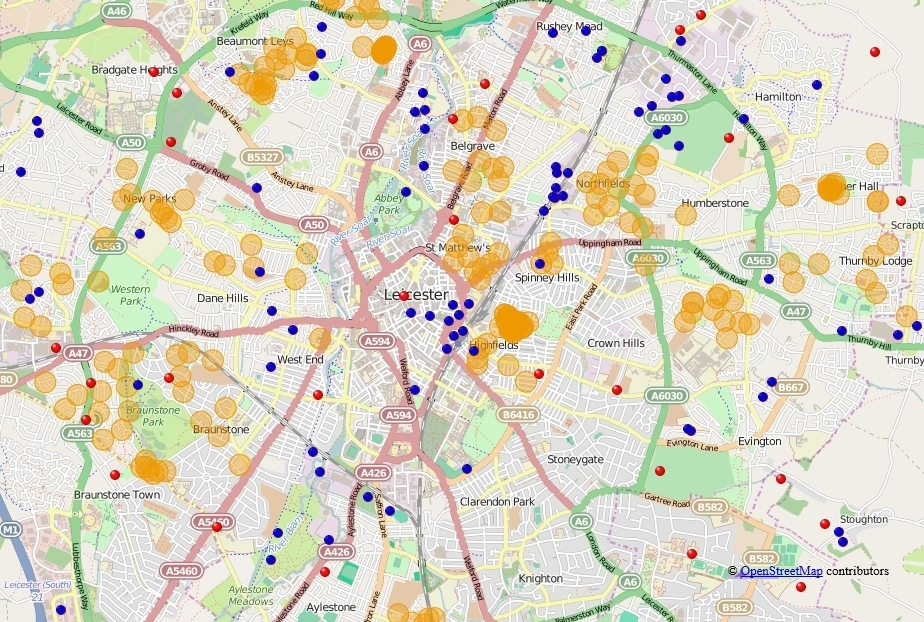
\includegraphics[width=\columnwidth]{images/viewsheds.jpg}
\caption{ CCTV viewsheds in the city of Leicester, UK}
\label{fig:viewsheds}
\end{figure} 

For our purposes, there are several ways that network data, that is,
vertices and edges, can be combined with geographical data. We applied
two methods, firstly with connectivity (edges) between vertices being
derived from viewsheds from individual vertices~\cite{gisruk:2015},
and secondly, a density calculation built directly into the social
network analysis measure of
\emph{betweenness}~\cite{oatley-et-al:2006a}. Our method thus combined
line of sight visibility (viewshed analysis) with techniques from
social network analysis to investigate this data. At increasing
distances different nodes are connected creating a set of networks,
which are subsequently described using centrality measures and
clustering coefficients. This technique has significant relevance to
CCTV cameras and their line of sight visibility, permitting
construction of different levels of possible network structures.

\subsection{Crime data}

The crime data was obtained from the UK's open data
repository\footnote{\url{http://data.police.uk}} for crime and
policing in England, Wales and Northern Ireland, which offers
street-level crime and outcome data for individual police forces and
neighbourhood teams. The UK’s Home Office published crime data
provided by the 43 geographic police forces in England and Wales, the
British Transport Police, the Police Service of Northern Ireland and
the Ministry of Justice. There are approximately four years of data
available, and the classification of crimes includes the following:
``{\emph{Anti-social behaviour}}'', ``{\emph{Bicycle theft}}'',
``{\emph{Burglary}}'', ``{\emph{Criminal damage and arson}}'',
``{\emph{Drugs}}'', ``{\emph{Other crime}}'', ``{\emph{Other
theft}}'', ``{\emph{Possession of weapons}}'', ``{\emph{Public
disorder and weapons}}'', ``{\emph{Public order}}'',
``{\emph{Robbery}}'', ``{\emph{Shoplifting}}'', ``{\emph{Theft from
the person}}'', ``{\emph{Vehicle crime}}'', ``{\emph{Violence and
sexual offences}}'', ``{\emph{Violent crime}}''.

\subsection{Social media data}

There are an increasing number of applications, services and
frameworks that will allow you to retrieve and analyse social data,
some for a fee, some available under academic licenses. We considered
the following sources of social media data for our
experiments:

\begin{itemize}
\item {\emph{GNIP}}\footnote{\url{http://gnip.com}} is a commercial company
that serves customers in over 40 countries who serve over 95\% of the
companies in the Fortune 500 with data from numerous social media
hosts, including Twitter, Tumblr, Foursquare, YouTube, Reddit,
Google+, Facebook and Instagram;
\item {\emph{Netlytic}}\footnote{\url{https://netlytic.org}} is a cloud-based
text and social networks analyser that can automatically summarise and
discover social networks from online conversations on social media
sites, allowing free access for up to three datasets per month from
Twitter (tweets matching a user specified query, including location,
tweeter and media used), Facebook (posts and replies from public
Facebook groups, pages, events, or profiles), Instagram and YouTube
(video comments);
\item {\emph{COSMOS}}\footnote{\url{http://www.cosmosproject.net/}}
(Collaborative Online Social Media Observatory) brings
together social, computer, political, health, statistical and
mathematical scientists to study the methodological, theoretical,
empirical and technical dimensions of social media data in social and
policy contexts~\cite{burnap-et-al:2015}. The open source tool
includes many pre-built packages for data mining and analysis,
including the ability to plot and view tweet locations on a
geo-spatial map.
\end{itemize}

After having various issues with securing access to the tools and
datasets presented above, we opted to use the data from the
{\emph{myPersonality}}
project\footnote{\url{http://myPersonality.org}}. {\emph{myPersonality}}
started out in June 2007 and collected Facebook data from the
{\emph{myPersonality}} `app' questionnaires, ending in 2012. Nearly
7.5m people have completed a questionnaire, with more than 40
countries having had 1000 or more participants (but
{\emph{myPersonality}} is only available in English); users are able
to retake {\emph{myPersonality}} tests (for example, one test -- the
{\emph{Big 5}} test -- has been retaken over 900,000 times), providing
longitudinal data. Users are able to rate the personalities of their
FB friends, with over 300,000 friend-ratings. About 40\% of users have
granted {\emph{myPersonality}} access to the data on their Facebook
profiles (this includes their preferences, as expressed by Facebook
Likes), providing more than 36,000,000 user-like
pairs~\cite{kosinski-et-al:2013}.

The list of variables is
extensive\footnote{\url{http://mypersonality.org/wiki/doku.php?id=list_of_variables_available}};
of particular interest to our current study include: demographic and
geo-location data (home and current location); religion, political
views, and profile about section; psychological profiles; Facebook
data; Facebook status updates; and, Facebook social
networks~\cite{kosinski-et-al:2013}. We were primarily interested in
the social media data, and the Big Five scores plus their constituent
facet scores, for all the users in the dataset. For example: the
number of posts on a user's wall ({\emph{n}}= 2057455; mean = 122.03;
SD = 318.48) -- there are 4077428 records in the {\emph{Big 5}} table,
with 3386778 unique respondents, and there are 38330 people for whom
both {\emph{Big 5}} and self-monitoring scores are available. So for
our purposes, we have personality traits, text from which we can
determine sentiment, relationship data, and a `triads' database
numbering more than 3.5 million entries, which can be used to study
dyads by ignoring the third actor. Unfortunately, the data or updates
are not geocoded, although there are recorded coordinates for `home'
and occasionally `current location'. When we attempted to use these
values, it drastically reduced the database down to a few hundred
compared to the original millions.

\subsection{Agent-based methodology}

Geospatial systems have long been paired with agent-based
models~\cite{gerritsen:2015}, for instance Crooks~\cite{crooks:2012}
with the digital representation and physical environment of cities,
along with Chorley, Whitaker \& Allen~\cite{chorley-et-al:2015} on
investigating personality and location-based social networks based on
check-in behaviour of volunteer Foursquare users. Crooks and
Castle~\cite{crooks+castle:2012} present a list of software and
guidelines for the integration of agent-based modelling and
geographical information for geospatial simulation; for the agent
simulation we used the {\emph{PyCX
Project}}\footnote{\url{http://pycx.sourceforge.net}} agent-based
modelling software.

Our experiments utilised the social media data from the
{\emph{myPersonality}} project; also friends, families, social network
analysis measures, personality traits, and our derived psychopathy
value. Our aim was to simulate the movement of many users in a city by
means of an agent-based model, and utilise the CCTV sensors in some
way to gain a measure of `ground-truth' or something to optimise
against. The primary idea was to see how we might be able to represent
these factors. Consider an agent, surrounded mainly by unknown people,
perhaps some friends or family, a number of happy people, a number of
sad people, the agent with their plans and beliefs, desires and
intentions; where do they move to? Consider the difficulty of
representing meaningful communication between agents in an
`unconstrained' environment, disambiguating (un)natural language,
automatic detection of events.


\section{Results}\label{res}

As we discussed previously, we derived a psychopathy score from the
{\emph{myPersonality}} dataset containing Five-Factors and subfactors,
but with such strong criteria we found no psychopaths (a good
result). We were therefore forced to successively `weaken' the
selection criteria, for instance
{\emph{Conscientiousness.SELF-EFFICACY}} being generalised from
`{\emph{Very low}}' to `{\emph{Low}}'. Within the data there were
approximately 7000 data points with all Five-Factors and subfactors,
and there were approximately 3 million data points with just the
Five-Factors. From c.7000 data points initially no users were
identified. Removing the {\emph{Neuroticism}} feature entirely, and
changing `{\emph{Very High}}' or `{\emph{Very Low}}' to
`{\emph{High}}'/`{\emph{Low}}', nine users were identified. Changing
all values to `{\emph{Medium}}' retrieved 66 users. From the 3 million
dataset, which does not include the subfactors, then ignoring these
1640 users were identified.

\begin{figure}[!htp]
\centering
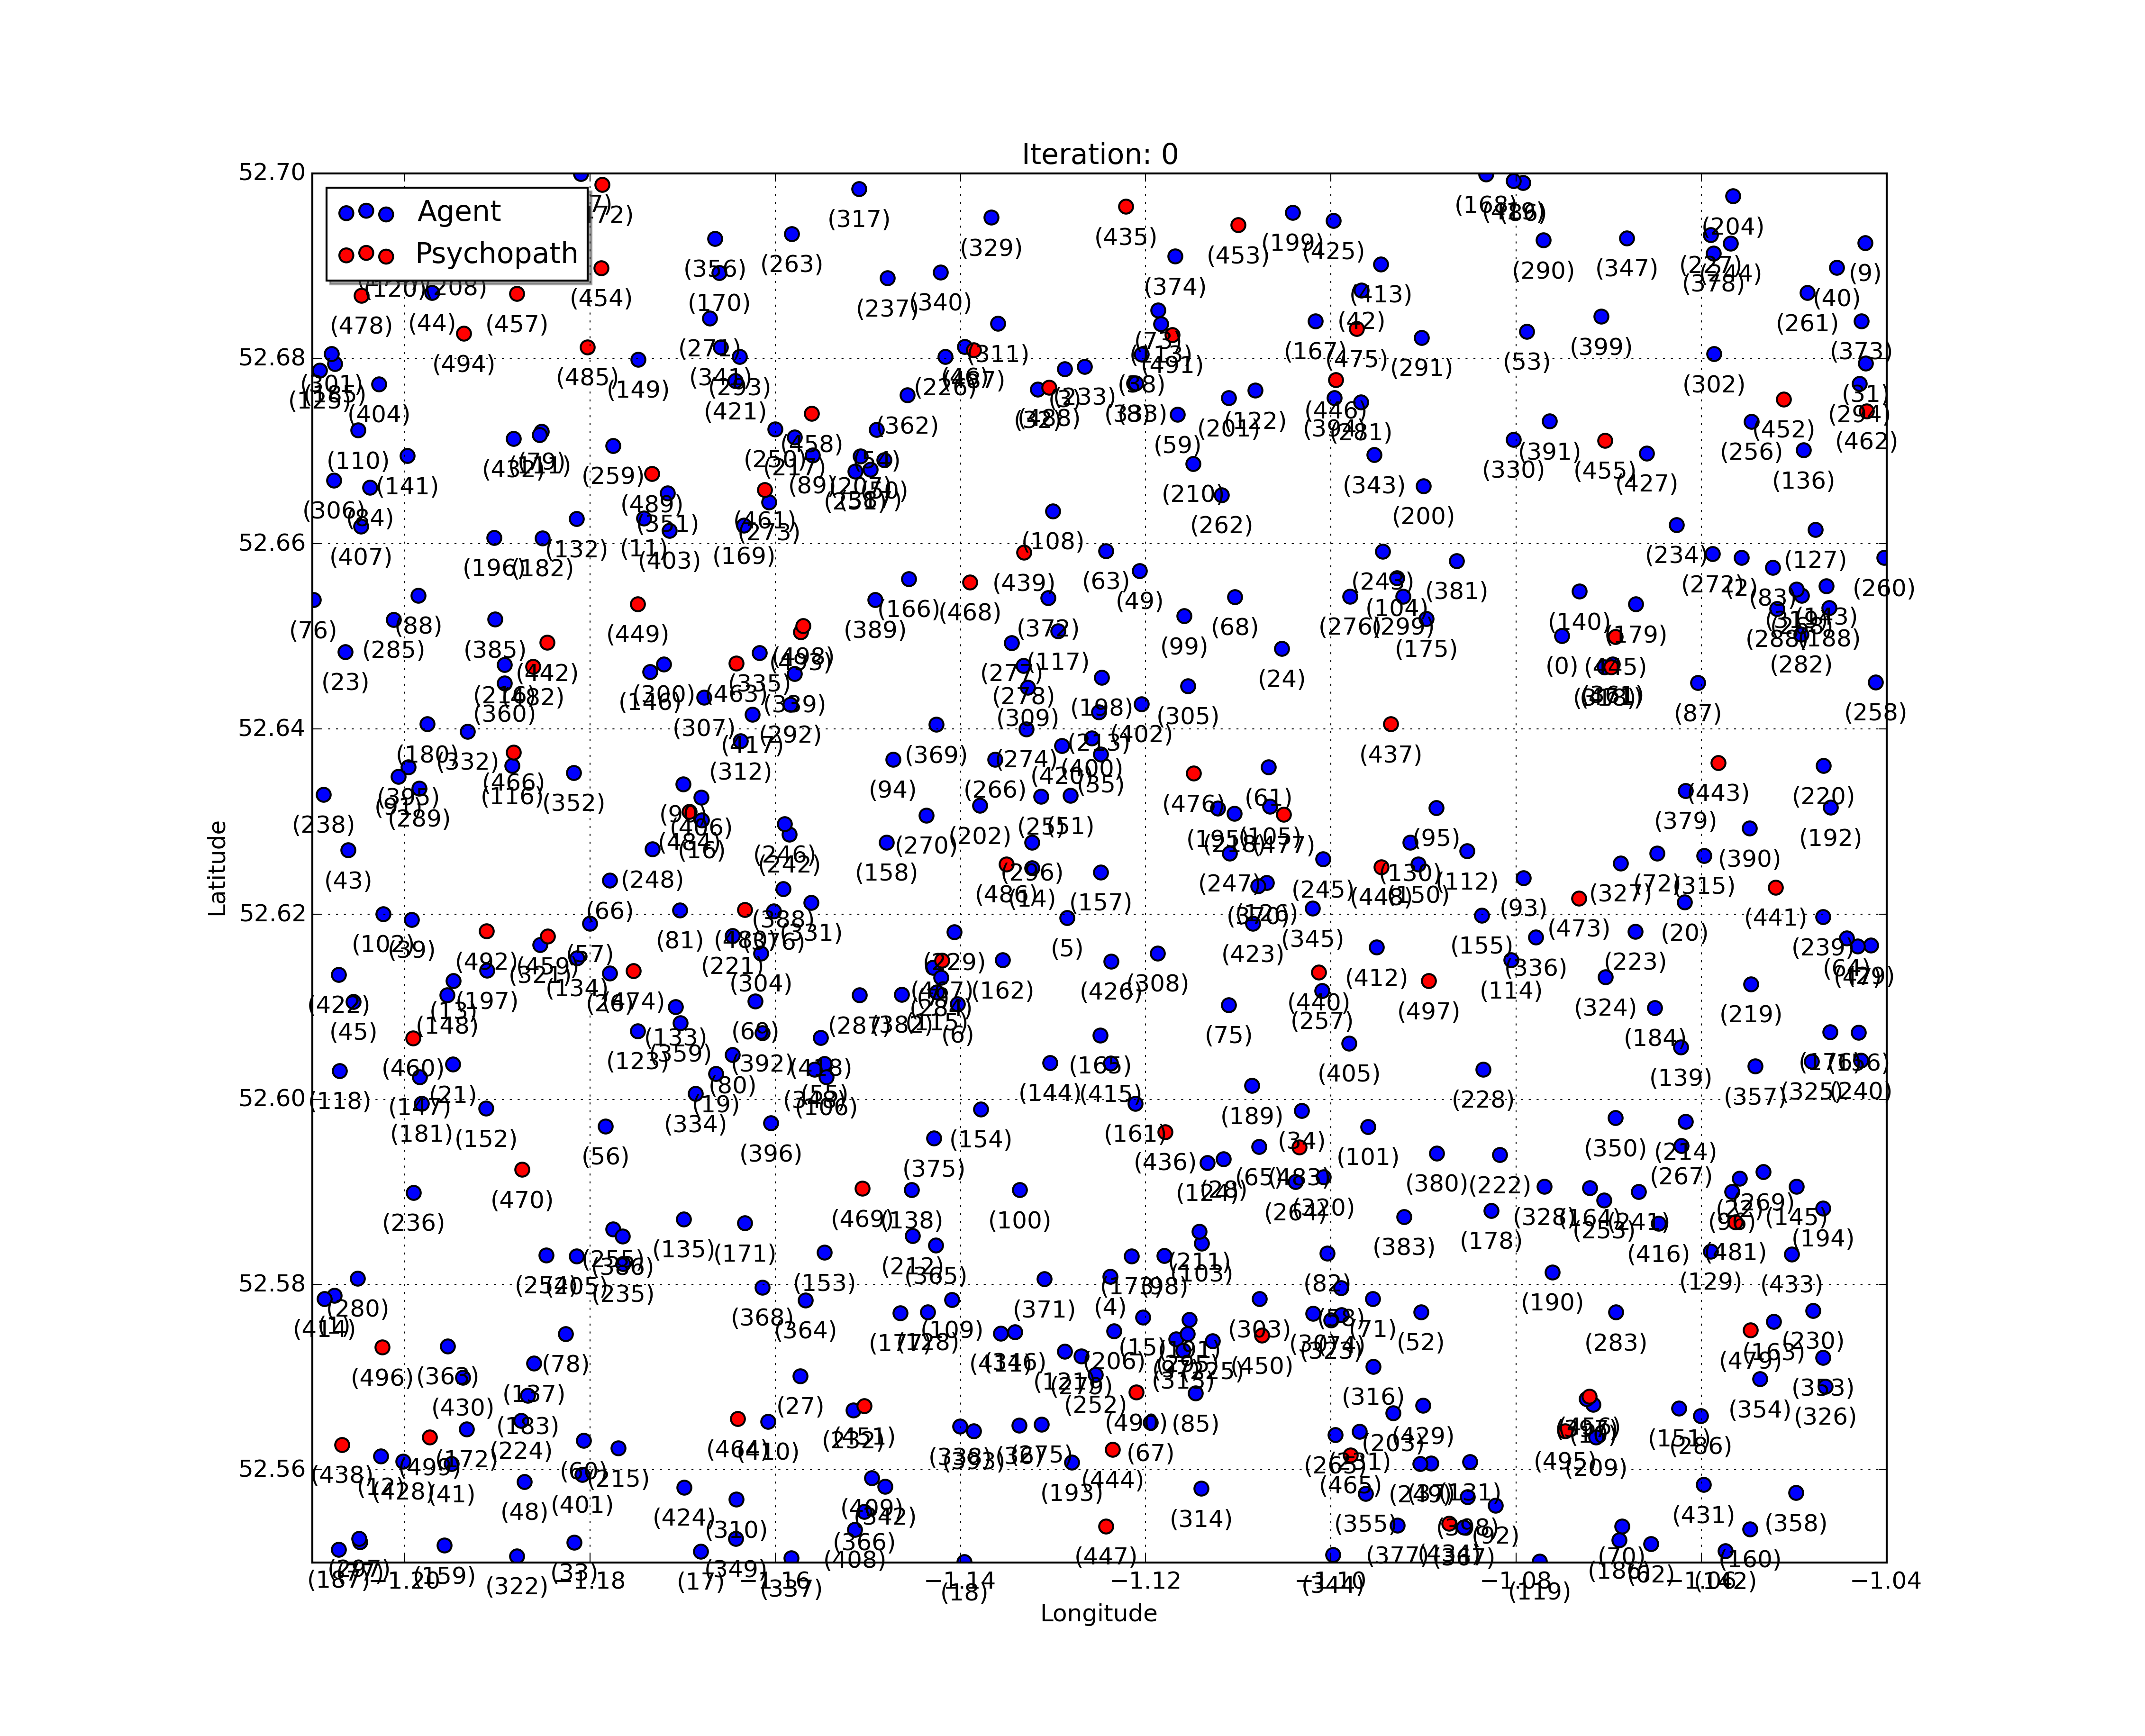
\includegraphics[width=\columnwidth]{images/Step_0_sim_11.png}
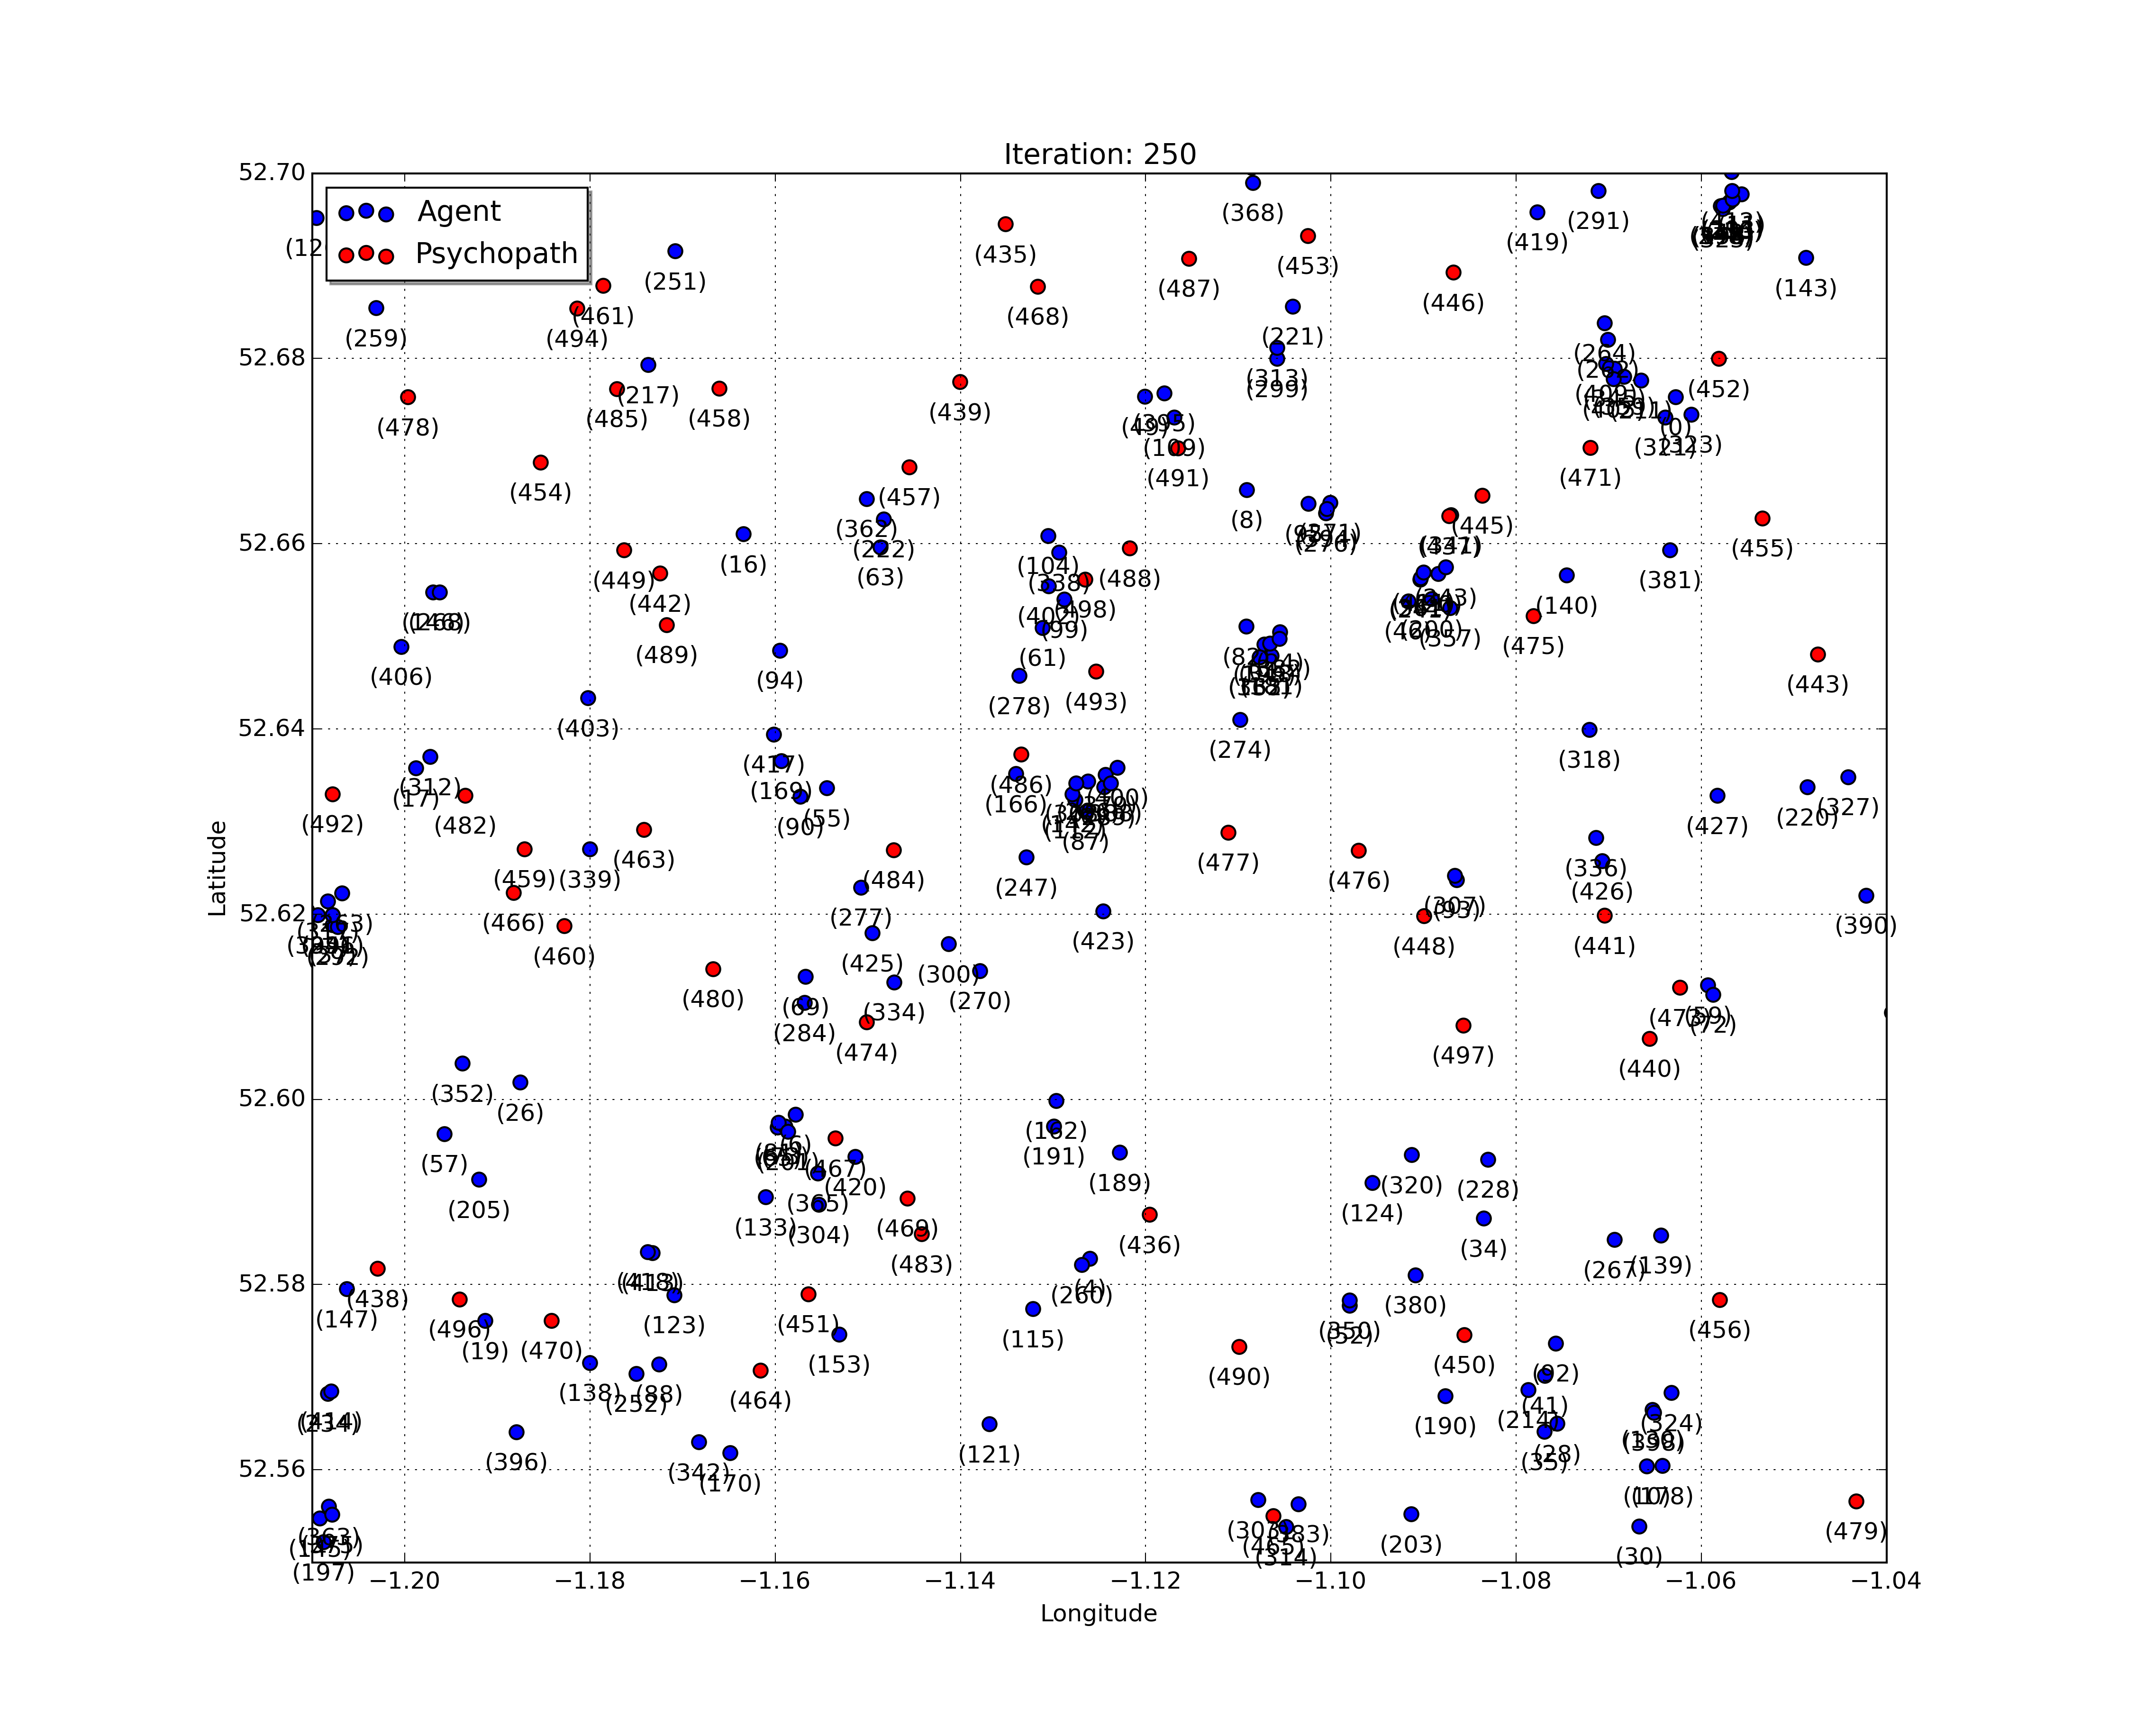
\includegraphics[width=\columnwidth]{images/Step_250_sim_11.png}
\caption{Agent start and finish positions. The data was comprised
  approximate equal numbers of psychopaths (using very weakened
  equations) and non-psychopaths. The reason for this was initially to
  build in other metrics of avoidance of CCTV and other criminal
  behaviour}
\label{fig:agentstartandfinish}
\end{figure}

We analysed all the data available for all
crimes in the city of Leicester, with increasing sizes of viewsheds
around the placement of CCTV cameras. Figure~\ref{fig:cctvcrimes}
shows viewsheds of sizes 10m, 100m and 200m, with the stacked
bar-chart showing the proportion of crimes in that year which were
within the respective viewsheds.

\begin{figure}[!htp]
\centering
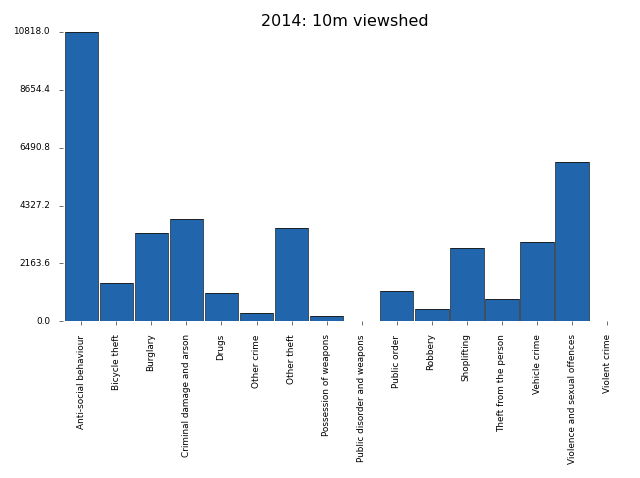
\includegraphics[width=\columnwidth]{images/2014-10m.png}
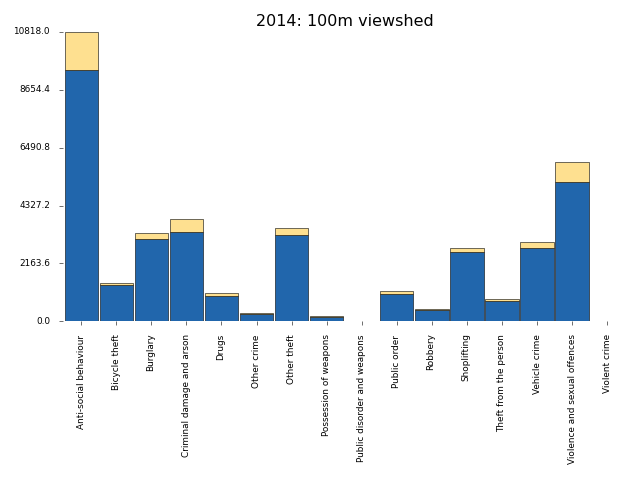
\includegraphics[width=\columnwidth]{images/2014-100m.png}
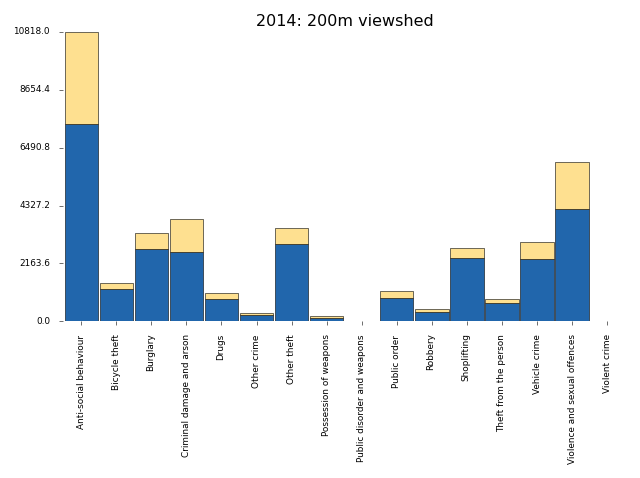
\includegraphics[width=\columnwidth]{images/2014-200m.png}
\caption{Proportion of crimes within CCTV viewsheds of 10m, 100m,
  200m. The features from left to right are the crimes of:
``{\emph{Anti-social behaviour}}'', ``{\emph{Bicycle theft}}'',
``{\emph{Burglary}}'', ``{\emph{Criminal damage and arson}}'',
``{\emph{Drugs}}'', ``{\emph{Other crime}}'', ``{\emph{Other
theft}}'', ``{\emph{Possession of weapons}}'', ``{\emph{Public
disorder and weapons}}'', ``{\emph{Public order}}'',
``{\emph{Robbery}}'', ``{\emph{Shoplifting}}'', ``{\emph{Theft from
the person}}'', ``{\emph{Vehicle crime}}'', ``{\emph{Violence and
sexual offences}}'', ``{\emph{Violent crime}}'' (full data available
from: \url{http://data.police.uk})}
\label{fig:cctvcrimes}
\end{figure}


\section{Discussion and Conclusions}\label{disc}

The technical issues surrounding smart CCTV, detecting crowd
characteristics indicative of disorder and violence, are those related
to image analysis and extracting crowd dynamics using motion
estimation techniques. Learning crowd characteristics is a significant
task without considering the problems caused by ambient weather
conditions, improper viewing angle, installation position, image
correction for lens distortion, and so on.  A major problem with many
CCTV installations is that the wrong lens is chosen, often resulting
in people being too small to successfully identify. Unless a camera
achieves `Recognition of a Known Person' it is unlikely to be used by
the police in the UK to identify a person for prosecution in a court
of law, and the police have stated that over 80\% of the video
evidence that they collect fails to meet the required standard.

CCTV offers the ability to validate or verify theories about
situations believed to be occurring derived from social media or other
digital sources. Therefore our interest in CCTV is as a sensor, that
can validate what is happening in the digital representation of a
city. The UK Home Office {\emph{CCTV Operational Requirements
Manual}}~\cite{ukhocctv:2009} prescribes the relevant technical
specifications. Camera and lens selections need to be chosen and based
upon a 1.7 metre person. Detection requires the image of the person
occupying at least 10\% of picture screen height on the monitor;
observation requiring 25\% screen height, to follow a group of people
such as in a town centre; recognition of a known person requires 50\%
screen height; and, identification of an unknown person requires 100\%
of picture screen height on the monitor. To observe a person at 50\%
(`Recognition of a Known Person') the CCTV can only view an area the
width of two car park spaces (4.3m). The most popular lens sold to
customers is a 1/3in (3.6mm) lens. This gives a wide angle view of
70\%, but can only provide facial recognition of 3.2m so if it is
located at a height of 5m it is no real use for recognition.

In general, there are too few cameras with too wide a field-of-view;
cameras can view a wide area, or provide a high-level of detail, but
not both. Many cameras are set to view an excessively large area
(possibly for cost-savings), which makes it impossible to positively
identify people at most points within the scene. Also, most cameras
installed today have fields of view that are set too wide to allow
facial recognition throughout most of their coverage area.

Utilising CCTV as a sensor to accurately model or give feedback on the
reality of occurrences in digital space currently has several
drawbacks, relating to both placement/position and quality of the
equipment to also the complexities of image analysis. Limitations of
our simulation include the lack of accurate/genuine geotagged data,
and from lack of information about CCTV cameras -- the UK city of
Leicester is one of the few with accurately recorded positions for a
study, but even of these we do not know the actual camera types (and
therefore the correct viewshed to use).

With many CCTV systems having sophisticated recording and real-time
logging/tracking capabilities, it raises wider questions about civil
liberties, privacy and data retention~\cite{goold:2002} --
particularly in light of anti-terrorist legislation in both the US
and UK~\cite{bowden:2002} -- despite numerous Freedom of Information
(FoI) requests to identify the specifics of systems in cities across
the UK. While there is significant potential for governments and
organisations to promote open and big data (for example, in supporting
effective policy-making~\cite{nesta:2015}), we raise the fact that it
is now clearly possible, and will in the future become more accurate,
that widespread data retention and aggregation could lead to abuses of
civil liberties. The recent re-positioning of public-private
partnerships in national cyber security strategies, particularly in
the US and UK~\cite{carr+crick:2015}, also raises questions
surrounding ambiguity of ownership, governance and
responsibility. Consider the lingering stigma of false accusations in
the press, or perhaps of being added in a gang-database (and never
removed), etc. We note the work of key organisations in this space,
such as the Electronic Frontier
Foundation\footnote{\url{https://www.eff.org/}} and the Open Rights
Group\footnote{\url{https://www.openrightsgroup.org/}}.

The results of the simulation are enough to demonstrate that many
forms of evidence, rich enough to describe the range from transient
moods to more permanent traits, can be derived from social media data;
CCTV is a form of validation of the event. As of yet there does not
exist a dataset that combines all of these features, for interest a
civil unrest dataset containing `live' geotagged tweets or status
updates, with accompanying CCTV feed. However this should not be too
far away, with CCTV set to become a commodity like other
utilities~\cite{graham:2002}, and smart CCTV touted as being able to
recognise the precursors for civil disobedience and riots.

The work of Schwartz et al.~\cite{schwartz-et-al:2013}
leverages what people say in social media to find distinctive words,
phrases, and topics as functions of known attributes of people such as
gender, age, location, or psychological characteristics. This can thus
be transposed, inferring gender, age and so on, from social media
data. The negative implications of these developments are that they
can easily be applied to large numbers of people without obtaining
their individual consent or even being aware. Commercial companies,
governmental institutions, or even one's Facebook friends could use
software to infer personality (and other attributes, such as
intelligence or sexual orientation) that an individual may not have
intended to share~\cite{lambiotte+kosinski:2014}.

Smart CCTV networks will need to consider more than just postures and
crowd positions, but also locations of unhappy or aggressive tweets or
Facebook status updates. Indeed, from sufficient (un)natural text it
is becoming possible to infer behaviours and even personality traits,
and we have demonstrated the first attempts to extend this recognising
psychopathy. Due to the explosive growth of cyber-real space and
crowds over the burgeoning social networking domains, the real space
in which we inhabit is also strongly tied with the virtual
cyber-social space. We are thus interested in understanding the
relationships and the interactions of crowds, in physical-real space
and cyber-social space.  By modelling areas in a landscape
(e.g. cities/urban domains) in terms of cyber-physical crowds who are
today commonly communicating through social networking, we expose
geotagged interactions. We can explore urban characteristics which are
reflected in the social networks through crowd behaviour.

We thus have a preliminary implementation of a model, with the
intention of being able to successfully model complex dynamics among
population, utilising features drawn from sources such as social media
updates, knowledge about friendship, networks, family, location. The
wider aims are broad; however initially we are interested merely to
develop our research ideas around representation.

%\newpage

% trigger a \newpage just before the given reference
% number - used to balance the columns on the last page
% adjust value as needed - may need to be readjusted if
% the document is modified later
\IEEEtriggeratref{59}
% The "triggered" command can be changed if desired:
%\IEEEtriggercmd{\enlargethispage{-5in}}

% references section
\bibliographystyle{IEEEtran}
\bibliography{dasc2015}

% that's all folks
\end{document}


